The lattice-QCD method is based on
regularising QCD on a finite Euclidean lattice and is generally
studied by numerical computation of QCD correlation functions in the
path-integral formalism, using methods adapted from statistical
mechanics.
%
To make contact with the physical world and experimental
data, the numerical results are extrapolated to the continuum 
and infinite-volume limits.
%
The past decade has seen significant progress in
the development of efficient algorithms for the generation of
ensembles of gauge field configurations, which represent the QCD
vacuum, and tools for extracting the relevant information from lattice-QCD
correlation functions.
%
In this respect, lattice-QCD calculations have reached a level where
they not only complement, but also guide current and forthcoming
experimental programs.

\subsubsection{Systematic uncertainties}
Lattice-QCD calculations must demonstrate control over all sources of
systematic uncertainty introduced by the discretisation of QCD on the
lattice to make meaningful contact with experimental data.
%
These
include discretisation effects that vanish in the continuum limit;
extrapolation from unphysically heavy pion masses; finite volume
effects; and renormalisation of composite operators.
%
To take the 
continuum limit requires accurate determinations of the lattice-spacing. 
We briefly review these main sources of systematic
uncertainty here; for a fuller account see, for
example, Ref.~\cite{Aoki:2016frl}.

\begin{itemize}

\item {\bfseries Discretisation effects and the continuum limit.} There is 
a fair degree of flexibility in discretizing the QCD action. This has
led to a variety of formulations, which differ mainly in the choice of
the action for quarks.
%
In the continuum limit, which corresponds to taking
the lattice spacing $a$ to zero with all physical quantities fixed,
the simplest discretisations differ from continuum QCD at ${\mathcal
O}(a)$.
%
In practice, one cannot afford to perform numerical
simulations at arbitrarily small lattice spacings, because the cost of
computation increases with a large inverse power of the lattice
spacing, and ${\cal O}(a)$ effects can be significant even
with current lattice spacings ranging from $0.15 \,\mbox{fm}$ to
$0.05 \,\mbox{fm}$.
%
To accelerate the convergence to the continuum
limit, improved quark and gluon actions are widely used, which include
higher-dimension operators to reduce the discretisation errors to
${\cal O}(a^2)$ or better.
%
Chiral fermions with automatic $\mathcal{O}(a)$ improvement and small 
$\mathcal{O}(a^2)$ discretisation errors are also adopted to admit 
calculations on coarser lattice spacings. 

\item {\bfseries Pion mass dependence.} 
The computational cost of the fermion contribution to the path
integral increases with a large inverse power of the bare quark mass
(or, equivalently, the pion mass).
%
Lattice-QCD calculations are therefore
often performed at unphysically heavy pion masses, although results calculated
directly with physical pion masses have become increasingly common, albeit with larger
errors.
%
To obtain results at the physical pion mass, lattice data are
generated at a sequence of pion masses and then extrapolated to the
physical pion mass.
%
To control the associated systematic
uncertainties, these extrapolations are guided by effective
theories.
%
In particular, the pion-mass dependence can be parametrized
using chiral perturbation theory ($\chi$PT), which accounts for the
Nambu-Goldstone nature of the lowest excitations that occur in the
presence of light quarks. 
%
With multiple lattices at different sea quark masses including some
at physical pion mass, several lattice spacings and volumes, one can  
perform global fits with judicious functional forms to determine
the final result at the physical pion mass and extrapolated continuum and 
infinite volumes.

\item {\bfseries Finite volume effects.} Numerical lattice-QCD 
calculations are necessarily restricted to a finite space-time
volume.
%
For most simple quantities, these effects decay exponentially
with the size of the lattice, and therefore the easiest way to
minimize or eliminate finite volume effects is to choose the volume
sufficiently large in physical units.
%
Unfortunately, this can be
prohibitively expensive as one approaches the continuum limit, requiring the
number of lattice sites to grow as $L/a$ in all four directions. 
%
Finite volume $\chi$PT is the preferred
tool to develop systematic expansions that provide quantitative
information on finite-volume effects.
%
In general, finite volume
effects of hadrons are dominated by their interactions with pions,
which can travel around the (periodic) lattice many times.
%
Numerical
evidence suggests that lattice sizes of $m_\pi L \geq 4$, where
$m_\pi$ is the pion mass, are generally sufficiently large that finite
volume effects are negligible for mesons, within the current precision 
of lattice-QCD calculations.
%
From the studies of the pseudoscalar and electromagnetic form factors of the 
nucleon, it is evident that larger physical volumes are needed for the 
baryons than those for the mesons.

\item {\bfseries Excited state contamination.} 
At small Euclidean times, a lattice-QCD correlation function
is a sum over a tower of states that behave as $e^{-m_it}$, where $m_i$ is the 
energy of the state and $t$ is the Euclidean time. 
%
Thus, at large Euclidean times,
ground-state quantities can be extracted by fitting to the dominant 
exponential behaviour.
%
Unfortunately, the signal-to-noise ratio is exponentially suppressed 
as $e^{-(E_N-3m_\pi/2)t}$, where $E_N$ is the nucleon energy and $m_\pi$ is the 
pion mass.
%
Thus, lattice-QCD results
are extracted from an intermediate region in which excited state contributions 
are either small or well-controlled and the signal-to-noise ratio is 
sufficiently large that the signal can be reliably extracted. 
%
This is a particular challenge for baryons and is one of the largest 
sources of systematic uncertainties for nucleon matrix elements.

\item {\bfseries Renormalisation.} The matrix elements extracted from a 
lattice-QCD calculation at a given lattice spacing are bare matrix elements,
rendered finite by the presence of the lattice spacing, which serves
as a gauge-invariant UV regulator. To take the continuum limit,
i.e. remove the regulator, one must renormalize the corresponding
operators and fields and match them to some common scheme and scale used 
by phenomenologists. Although renormalisation is traditionally
discussed in the framework of perturbation theory, at hadronic energy
scales the renormalisation constants should be computed
nonperturbatively to avoid uncontrolled uncertainties due to 
truncated perturbative results.
%
In QCD with only light quarks it is technically
advantageous to employ so-called mass-independent renormalisation
schemes.
%
This requires a renormalisation condition that can be
implemented on the lattice as well as in continuum perturbation
theory. A common choice is the regularisation-independent/momentum (RI/MOM) 
scheme~\cite{Martinelli:1994ty}.

In addition, on a hyper-cubic lattice, the orthogonal group $O(4)$ of
continuum Euclidean space-time is reduced to the hyper-cubic group
$H(4)$.
%
Thus, operators are classified according to irreducible
representations of $H(4)$~\cite{Gockeler:1996mu}.
%
Different
irreducible representations belonging to the same $O(4)$ multiplet
will, in general, give different answers at finite lattice spacing, an
effect that can be reduced by improving the
operators~\cite{Gockeler:2004wp}.
%
Conversely, operators that lie in
different irreducible representations of $O(4)$, but the same irreducible
representations of $H(4)$, will mix at finite lattice spacing but not
in the continuum. When these operators have lower mass dimensions,
the mixing coefficients scale with the inverse lattice spacing to some
power, and diverge in the continuum limit.
%
This power-divergent mixing
must be removed nonperturbatively, and is a particular challenge for
lattice calculations of the Mellin moments of PDFs (see
Sect.~\ref{Sec:MomentsLQCD}).

Finally, it is worth noting that factorization, the key assumption of
the operator product expansion (OPE), demands that the nonperturbatively 
renormalised hadron matrix elements are matched to the perturbatively 
renormalised Wilson coefficients at a scale where the perturbative 
expressions show convergence. This appears to be
the case for scales $\mu^2 \gtrsim 10\mbox{ GeV}^2$ at
least~\cite{Gockeler:2010yr}. This, however, is a fundamental aspect
of QCD, and is not restricted to lattice QCD. The DGLAP evolution equations,
for example, work best for $q^2_{\rm min} \approx
15\mbox{ GeV}^2$~\cite{Abramowicz:2015mha}, which should be kept in
mind when comparing lattice results with phenomenology.

\item {\bfseries Lattice-spacing determination.} 
Numerical lattice-QCD calculations 
naturally determine all dimensionful quantities in units of the
lattice spacing. Thus, extracting physical values requires the
determination of the lattice scale. This is achieved by matching a
quantity with mass-dimension to its experimental value or through a
well-defined theoretical procedure, that is referred to as
``scale-setting''. Popular reference scales include light decay
constants, hadron masses, scales defined in terms of the heavy quark
potential or, most recently, the length scale $\sqrt{t_0}$~\cite{Luscher:2010iy} and $w_0$~\cite{Borsanyi:2012zs} defined via the Wilson 
gradient flow~\cite{Luscher:2010iy} have become very popular scale setting methods. These scales can be computed cheaply and can be used to very accurately
match scales between different gauge ensembles.  However, a hadron mass or a decay constant which are known accurately by experiment and can be computed precisely in lattice-QCD have to be used for absolute scale setting. A popular hadronic mass for this purpose is the mass of the triply strange $\Omega$ baryon~\cite{Durr:2008zz} or the 2S-1S splitting in the Upsilon spectrum~\cite{Kendall:2008zz}.

\end{itemize}

These sources of systematic uncertainty all need to be under control
when confronting experimental data with lattice results, or vice
versa.
%
For a coherent assessment of the present state of lattice-QCD
calculations of various quantities, the degree to which each
systematic has been controlled in a given calculation is an important
consideration.
%
Therefore, in the following sections, we indicate the
quality of the lattice calculations, based on criteria inspired by the
FLAG analysis of flavor physics on the lattice~\cite{Aoki:2016frl}.

\subsubsection{Mellin moments of PDFs from lattice QCD}
\label{Sec:MomentsLQCD}

PDFs cannot be directly determined in Euclidean lattice QCD, because their 
field-theoretic definition involves fields at light-like separations.
%
Instead, 
the traditional approach for lattice-QCD calculations has been to determine the matrix elements of local twist-two operators, where twist is the dimension minus the spin, that can be related to the Mellin moments of PDFs.
%
In principle, given a sufficient number of Mellin moments, PDFs can be reconstructed from the inverse Mellin transform. In practice, however, the calculation is limited to the lowest three moments, because power-divergent mixing occurs between twist-two operators on the lattice.
%
Three moments are insufficient to fully reconstruct the momentum dependence of the PDFs without significant model dependence~\cite{Detmold:2003rq}.
%
The lowest three moments do provide, however, useful information, both as benchmarks of lattice-QCD calculations and as constraints in global extractions of PDFs. Here we briefly review the determination of Mellin moments of PDFs from lattice QCD. 

Using the OPE, the Mellin moments of structure functions, and the corresponding PDFs, can be expressed, up to higher twist effects, in terms of matrix elements of local operators:
\begin{align}
\!\!\!2 \int_0^1 dx\, x^{n-1} F_1(x,Q^2) &= \sum_a C_{1,a}^n(\mu^2)\, v_a^n(\mu^2)|_{\mu^2=Q^2} = \sum_a C_{1,a}^n(\mu^2)\, \int_0^1 dx\, x^{n-1} f_a(x,Q^2)\,,\\
4 \int_0^1 dx\, x^n g_1(x,Q^2) &= \sum_a e_{1,a}^n(\mu^2)\, a_a^n(\mu^2)|_{\mu^2=Q^2} = \sum_a e_{1,a}^n(\mu^2)\, \int_0^1 dx\, x^n\, 2 \Delta f_a(x,Q^2)\,,
\end{align}
where $v_i^n(\mu^2)$ and $a_i^n(\mu^2)$ are reduced matrix elements of the appropriate twist-two operators~\cite{Gockeler:1995wg},
\begin{align}
\frac{1}{2} \sum_s \langle p,s|\mathcal{O}^i_{\{\mu_1,\cdots,\mu_n\}}|p,s\rangle = {} & 2 v_i^n\, [p_{\mu_1}\cdots p_{\mu_n} - {\rm traces}] \,, \label{eq:twist2me}\\
\langle p,s|\mathcal{O}^{5\,i}_{\{\sigma \mu_1,\cdots,\mu_n\}}|p,s\rangle = {} & \frac{1}{n+1} a_i^n\, [s_\sigma p_{\mu_1}\cdots p_{\mu_n} - {\rm traces}]\,,
\end{align}
and $C_{1,i}^n(\mu^2)$ and $e_{1,i}^n(\mu^2)$ are the Mellin moments of the corresponding Wilson coefficients
\begin{equation}
C_{1,i}^n(\mu^2) = \int_0^1 dy\, y^{n-1} c_{1,i}(y,\mu^2)\,, \quad
e_{1,i}^n(\mu^2) = \int_0^1 dy\, y^n e_{1,i}(y,\mu^2)\,.
\end{equation}
The trace terms include operators with at least one factor of the metric tensor $g^{\mu_i \mu_j}$ multiplied by
operators of dimension $(n+2)$ with $n-2$ Lorentz indices. The operators relevant for the lowest two moments are listed in Table \ref{Tab:twist2}. The operator $\mathcal{O}^q_{\mu_1\mu_2}$ decomposes into two different representations of $H(4)$~\cite{Gockeler:1996mu}, each with different lattice artifacts and renormalisation factors. In the continuum limit, however, both operators should lead to the same result. In contrast, the operator $\mathcal{O}^q_{\mu_1\mu_2\mu_3}$ 
splits into several representations of $O(4)$ transforming identically 
under $H(4)$, causing the corresponding operators to mix under renormalisation 
on the lattice.

%%%%%%%%%%%%%%%%%%%%%%%%%%%%%%%%%%%%%%%%%%%%%%%%%%%%%%%%%%%%%%%
\begin{table}
\renewcommand{\arraystretch}{1.6} 
\centering
\begin{tabular}{@{}ccc@{}}
\hline 
Matrix element & Operator & PDF moment \\ 
\hline
$v_q^2$\,, $v_{\bar{q}}^2$  & 
$\displaystyle \left({\rm i}/2\right) \bar{q}(x)\gamma_{\mu_1} \overleftrightarrow{D}_{\mu_2} q(x)$ & 
$\langle x \rangle_{q^+}$\\
$v_q^3$\,, $v_{\bar{q}}^3$  & $\displaystyle \left({\rm i}/2\right)^2 \bar{q}(x)\gamma_{\mu_1} \overleftrightarrow{D}_{\mu_2} \overleftrightarrow{D}_{\mu_3} q(x)$ & $\langle x^2 \rangle_{q^-}$\\
$a_q^0$ & $\displaystyle \bar{q}(x)\gamma_{\sigma} \gamma_5 q(x)$ & 
$2\, \langle 1 \rangle_{\Delta q^+}$ \\
$a_q^1$ & $\displaystyle \left({\rm i}/2\right) \bar{q}(x)\gamma_{\sigma} \gamma_5 \overleftrightarrow{D}_{\mu_1} q(x)$ & $2\, \langle x \rangle_{\Delta q^-}$ \\
$v_g^2$ & $\displaystyle - {\rm Tr}\, F_{\mu_1\alpha}F_{\mu_2\alpha}$ & $\langle x \rangle_g$ \\
\hline
\end{tabular}
\caption{\label{Tab:twist2}
\small List of operators relevant for
the computation of the lowest two Mellin moments of polarised and unpolarised PDFs.
%
Here we indicate, for each operator, the corresponding matrix element and
the specific PDF moment that can be evaluated (see
Appendix~\ref{app:notation} for the notation used).
}
\end{table}
%%%%%%%%%%%%%%%%%%%%%%%%%%%%%%%%%%%%%%%%%%%%%%%%%%%%%%%%%%%%%%%

\paragraph*{Higher-twist contributions.}
%
The discussion so far has focused on the limit in which higher-twist contributions, suppressed by powers of the momentum-transfer, have been ignored. In fact, higher twist contributions to the lowest moment of the structure function $F_1(x,Q^2)$ are found to be of ${\cal O}(1\mbox{ GeV}^2/Q^2)$~\cite{Blumlein:2008kz}.
%
For lattice QCD, typically $Q^2 \simeq 1/a^2$, and at present lattice spacings this corresponds to $Q^2 = {\cal O}(10\mbox{ GeV}^2)$ or a higher-twist contribution of $5 - 10\, \%$. With contributions of higher-twist included, the OPE reads
\begin{equation}
2 \int_0^1 dx\, x F_1^q(x,Q^2) = C_{1,q}^2(\mu^2)\, v_q^2(\mu^2)|_{\mu^2=Q^2} + \frac{\bar{C}_{1,q}^2(\mu^2)}{Q^2}\, \bar{v}_q^2(\mu^2)|_{\mu^2=Q^2} + \cdots \,,
\label{tex}
\end{equation}
where $\bar{C}_{1,q}^2$ and $\bar{v}_q^2(\mu^2)$ are the Wilson coefficient and reduced matrix element of a generic twist-four operator. Both twist-two and four contributions mix under renormalisation, to the extent that the perturbative series for the Wilson coefficients $C_{1,q}^2(\mu^2)$ diverges due to the presence of IR renormalon singularities.
%
This ambiguity is canceled by that in the twist-four matrix element $\bar{v}_q^2(\mu^2)$ that arises as a result of an UV renormalon singularity~\cite{Martinelli:1996pk}. If mixing effects are ignored, the uncertainties will be, at least, comparable to the power corrections themselves.
%
Power corrections can be assessed most efficiently, and the twist expansion tested, by a direct lattice-QCD evaluation of the Compton amplitude, which we discuss in Sect.~\ref{Sec:InversionMethod}.

\paragraph*{Beyond the first three moments.}
%
Moving beyond the lowest three moments requires overcoming the challenge of power-divergent mixing for lattice-QCD twist-two operators.
%
One novel approach to this problem~\cite{Davoudi:2012ya} builds upon the physical intuition that as long as the scale associated with the operator (for the twist-two operators, this is the renormalisation scale $\mu$) is taken to be much larger than the hadronic scale but much smaller than the inverse lattice spacing, no singularity necessarily arises as one takes the continuum limit.
%
The operator can still probe the correct hadron structure at the scale $\mu$, but should be insensitive to the details of the discretisation of the operator at shorter distances.
%
A simple way to incorporate an intrinsic ``smearing'' scale for an operator is to sum over bilinears of quark fields that are displaced over many lattice sites in a small (compared to the scale $1/\mu$) region of Euclidean space-time (an alternative approach appears in~\cite{Monahan:2015lha}).


To ensure that the correct $SO(4)$ transformation properties of the matrix elements are recovered in the continuum limit, one must project the sum using hyper-spherical harmonics.
%
The properties of these operators, such as their mixing patterns and scaling properties, are discussed in detail in
Ref.~\cite{Davoudi:2012ya}.
%
In particular, while the classical mixing with lower and higher spin operators are both suppressed by $\sim a^2$ for spatially improved operators, the mixing at one-loop in lattice perturbation theory is suppressed by ${\cal O}(\alpha_s a)$ or ${\cal O}(\alpha_s a^2)$, depending on the lattice action used and provided that the gauge links used in constructing the gauge-invariant bilinears are tadpole-improved and smeared over a region whose physical size is held fixed as the continuum limit is taken. In principle, this allows higher moments of PDFs to be obtained from lattice QCD, without power-divergences. Numerical investigations of this approach,
which requires gauge configurations with very fine lattice spacings, are underway.

\subsubsection{The $x$-dependence of PDFs from lattice QCD}
\label{sec:xdependence}

While the lowest three moments of PDFs provide important benchmarks for lattice-QCD calculations of nucleon structure, and useful constraints in global extractions of PDFs, they are not in themselves sufficient to determine the $x$-dependence of PDFs, particularly at small $x$.
%
In the following section we summarize recent approaches to determining the $x$-dependence of PDFs directly from lattice QCD.

\paragraph*{Hadronic tensor.} 
PDFs can, in principle, be extracted from hadronic tensors provided the 
higher-twist contributions, which have different $Q^2$ dependence than the 
leading twist, can be subtracted. 
%
Calculating the hadronic tensor in the Euclidean path-integral approach
has the advantage that no renormalisation is required if conserved vector      
currents are used in the current-current correlation and only finite 
renormalisations are needed for the local currents.
%
Furthermore, since the structure functions are frame-independent, they 
can be calculated in any momentum frame of the nucleon. 
%
One can choose the nucleon momenta and momentum transfers judiciously 
to have a desirable coverage of $x$ for a given $Q^2$. 
%
However, the inverse Laplace transform which is needed to convert the hadronic tensor from Euclidean space to Minkowski space can be a 
challenge~\cite{Liu:1993cv,Liu:1999ak}. 
%
Three numerical approaches, the Backus-Gilbert method~\cite{Hansen:2017mnd}, 
improved maximum entropy, and fitting with model spectral functions, 
are suggested to tackle this inverse Laplace-transform 
problem~\cite{Liu:2016djw}. 
%
Ref.~\cite{Liu:1993cv} separates sea partons into ``connected sea'' and 
``disconnected sea'' contributions, based on the distinct topologies of the 
diagrams in a lattice computation. 
%
This​ ​distinction​ ​can​ ​help​ ​identify​ ​the​ ​impact​ ​on​ ​PDF​ ​uncertainties​ ​of​ ​
improving the​ ​uncertainties​ ​associated​ ​with​ ​disconnected​ ​diagrams​ ​determined​ ​
using​ ​lattice-QCD.
%
The extended evolution equations to accommodate both the connected sea 
(CS) and disconnected sea (DS) partons are derived~\cite{Liu:2017lpe}.
%
It is essential to have separately evolved CS and DS partons so that 
comparison with lattice calculations of unpolarised and polarised moments of
PDFs can be made. 
%
Only with the extended evolution equations will the CS and DS partons 
remain separated at different $Q^2$ to facilitate global fitting 
of PDFs with separated CS and DS partons.

\paragraph*{The inversion method.} 
\label{Sec:InversionMethod}

The Compton amplitude $T_{\mu\nu}(p.q)$, Eq.~(\ref{eq:Compton}) can be
directly obtained in lattice QCD, including disconnected contributions,  by a simple extension~\cite{Chambers:2017dov} of existing implementations of the Feynman-Hellmann technique to lattice QCD~\cite{Horsley:2012pz,Chambers:2014qaa,Chambers:2015bka}.
%
Provided one works at sufficiently large $Q^2$, the Compton amplitude will be dominated by twist-two contributions.
%
Varying $Q^2$ allows one to test the twist expansion and, in particular, isolate twist-four contributions. Moreover, one can distinguish between contributions from up, down and strange quarks, connected and disconnected, by appropriate insertions of the electromagnetic current.

To compute the Compton amplitude from the Feynman-Hellmann relation, a perturbation to the QCD Lagrangian is introduced, for example,
\begin{equation}
\mathcal{L}(x) \rightarrow \mathcal{L}(x) + \lambda \mathcal{J}_3(x)\,, \quad \mathcal{J}_3(x)=Z_V\cos(\vec{q}\vec{x})\; e_q \,\bar{q}(x)\gamma_3 q(x) 
\label{in}
\end{equation}
where $q$ is the quark field to which the photon is attached, and $e_q$ its electric charge. For simplicity, we consider the local vector current only, so that the renormalisation factor $Z_V$ is known and no further renormalisation is needed. Taking the second derivative of the nucleon two-point function 
\begin{equation}
\langle N(\vec{p},t) \bar{N}(\vec{p},0)\rangle_\lambda \simeq C_\lambda\, {\rm e}^{-E_\lambda(p,q)\,t}
\end{equation}
with respect to $\lambda$ on both sides, gives
\begin{equation}
-2 E_\lambda(p,q)\, \frac{\partial^2}{\partial\lambda^2}  E_\lambda(p,q)\,\big|_{\lambda=0} = T_{33}(p,q) \,.
\end{equation}
For $p_3=q_3=q_4=0$ this leaves us with
\begin{equation}
T_{33}(p,q) = 4 \omega^2 \int_0^1 dx\,  \frac{xF_1(x,Q^2)}{1-(\omega x)^2} \,.
\label{ff}
\end{equation}
Note that to extract the polarised structure functions requires insertions of two different currents with $\mu\neq \nu$. The idea is then to solve Eq.~\eqref{ff} for $F_1(x,Q^2)$ numerically.
%
In~\cite{Ji:2001wha,Chambers:2017dov} it was shown that the unpolarised 
structure function $F_1(x,Q^2)$ can be computed from a lattice calculation 
of the Compton amplitude, devoid of any renormalisation and mixing issues. 
%Furthermore, by extending the calculation to values $\omega > 1$ 
%it becomes possible to compute the structure functions down to fractional 
%momenta $x = {\cal O}(0.001)$. 
With the same method, PDFs can be computed directly without the need to go 
through the structure functions, provided $Q^2$ is sufficiently large that 
power corrections can be neglected. 

\paragraph*{Quasi-PDFs.}
Quasi-PDFs provide an alternative approach to determining the $x$-dependence of PDFs directly from lattice QCD~\cite{Ji:2013dva,Ji:2014gla}. In the following discussion, we focus on the flavor-nonsinglet quasi-PDF, for which we can ignore mixing with the gluon quasi-PDF. The unpolarised quark quasi-PDF is defined as the momentum-dependent
nonlocal forward matrix element
\begin{align}\label{eq:qPDF}
\widetilde{q}(x,\Lambda,p_z)  = {} &  \int \frac{dz}{2\pi} e^{-i x z p_z} p_z h(z,p_z), \nonumber \\
h(z,p_z) = {} &
\frac{1}{4 p_{\alpha}}\sum_{s=1}^2\left\langle p,s\right\vert \bar{\psi}(z)\gamma_\alpha e^{ig\int_0^z
A_z(z^\prime) dz^\prime} \psi(0) \left\vert p,s\right\rangle,
\end{align}
where $\Lambda$ is an ultraviolet (UV) cut-off scale, such as the inverse lattice spacing $1/a$. The Lorentz index $\alpha$ of the matrix $\gamma_\alpha$ has generally be chosen to be spatial, $\alpha = z$, but the alternative choice $\alpha = 4$ is also possible and removes part of the leading order twist-4 contamination~\cite{Xiong:2013bka,Radyushkin:2016hsy}. 
%\Blue{(JWC: Choosing $\alpha = 4$ eliminates a term that is purely higher-twist, but the remaining term still has a higher-twist effect. This can be seen easily from OPE.)} 
Note that, because $p$ is finite, the momentum fraction $x$ can be larger than unity.

The quasi-PDF is defined for nucleon states at finite momentum and must be related to the corresponding light-front PDF\footnote{In this context the term light-front PDF is used to distinguish PDFs from quasi-PDFs}, for which the nucleon momentum is taken to infinity.
In the  large-momentum  effective field theory (LaMET) approach, the quasi-PDF $\widetilde{q}(x,\Lambda,p_z)$ can be related to the $p_z$-independent
light-front PDF $q(x,Q^2)$ through~\cite{Ji:2013dva,Ji:2014gla}
\begin{equation} \label{eq:qPDFmatching}
\widetilde{q}(x,\Lambda ,p_z) = 
  \int_{-1}^1 \frac{dy}{\left\vert y\right\vert} 
    Z\left( \frac{x}{y}, \frac{\mu}{p_z}, \frac{\Lambda}{p_z}\right)_{\mu^2 = Q^2} q(y,Q^2) +
  \mathcal{O}\left( \frac{\Lambda_\text{QCD}^2}{p_z^2},\frac{M^2}{p_z^2}\right), 
\end{equation}
where $\mu$ is the renormalisation scale;
$Z$ is a matching kernel; and $M$ is the nucleon mass.
Here the $\mathcal{O}\left(M^2/p_z^2\right)$ terms are target-mass corrections and the $\mathcal{O}\left(\Lambda_\text{QCD}^2/p_z^2\right)$ terms are higher twist effects, both of which are suppressed at large nucleon momentum. A complementary approach to LaMET views the quasi-PDF as a ``lattice cross-section'' from which the light-front PDF can be factorised~\cite{Ma:2014jla,Ma:2014jga,Ma:2017pxb} and an alternative, but related, construction is proposed in Refs.~\cite{Radyushkin:2016hsy,Radyushkin:2017cyf} and explored in Ref.~\cite{Orginos:2017kos}.

\begin{comment}
To understand the origin of the power-suppressed corrections, we apply the OPE to the matrix element that defines the PDF, which becomes a linear combination of local twist-2 operators, with matrix elements in the proton state given by Eq.~\eqref{eq:twist2me}. From this it follows that the light-cone correlation function is {\it kinematically} connected with the +-components of the nucleon four-momentum. To eliminate the time dependence, we consider matrix elements of twist-two operators with $\mu_1=\mu_2=...=\mu_n=z$ and nucleon states with large $p_z$, to give
\begin{equation}
\frac{1}{2} \sum_s \langle p,s|\mathcal{O}^i_{\{z,\cdots,z\}}|p,s\rangle = 2v_i^n(\mu^2)\left[p_z^n-\lambda M^2 p_z^{n-2}-...\right], 
\end{equation}
where $\lambda$ is a number of order unity, and the ellipsis represents terms
with still lesser powers of $p_z$. Lorentz symmetry guarantees that the matrix elements of the trace terms are at most
$p_z^{n-2}$ times $\Lambda^2_{\rm QCD}$. \footnote{Ref.~\cite{Rossi:2017muf} argues that the trace terms are actually $p_z^{n-2}$ times $a^{-2}$; hence, these twist-4 terms are not suppressed. Later, Ref.~\cite{Ji:2017rah} shows that these dangerous terms will not appear once the matrix element is renormalised.}
 Thus, we conclude that
\begin{equation}
      \langle p| {\overline \psi}\gamma_ziD_z ... iD_z \psi|p\rangle
       = 2v^n(\mu^2) p_z^n\times \left[ 1 + {\cal O}\left(\frac{\Lambda^2_{\rm QCD}}{p_z^2},  \frac{m^2}{p_z^2}\right)\right],
\end{equation}
where the non-leading terms are power-suppressed in the large $p_z$ limit. Equating the renormalised moments on the right hand side of this equation with those that appear above
leads to the relation between the quasi-PDF and the light-front
PDF expressed in Eq.~\eqref{eq:qPDFmatching}.
\end{comment}


Preliminary results from lattice calculations of quasi-PDFs have been encouraging~\cite{Lin:2014zya,Alexandrou:2015rja,Chen:2016utp,Alexandrou:2016jqi}, as we illustrate in Fig.~\ref{fig:qPDF-demo}. There are a number of remaining challenges, however, that must be overcome for an {\it ab initio} determination of the $x$-dependence of PDFs directly from lattice QCD that incorporates complete control over systematic uncertainties. Lattice calculations of quasi-PDFs are subject to the same sources of systematic uncertainty that plague all lattice calculations and are highlighted in Sect.~\ref{Sec:IntroLQCD}, but here we focus on systematic uncertainties that are more specific to quasi-PDFs. These are uncertainties associated with the finite nucleon momentum of the lattice calculations and with the renormalisation of quasi-PDFs.

\begin{itemize}
 \item Preliminary nonperturbative studies of the quasi-PDF used nucleon momenta in the range $p_z = 2\pi/L$ to $10\pi/L$, where $L$ is the physical extent of the lattice, corresponding to $p_z = 0.5$ to $2.5$~GeV~\cite{Lin:2014zya,Alexandrou:2015rja,Chen:2016utp,Alexandrou:2016jqi}. At such low momenta, higher-twist and target mass corrections are likely to be considerable.

Target mass corrections can be removed to all orders~\cite{Chen:2016utp}, and twist-4 contributions can be removed in principle~\cite{Chen:2016utp,Radyushkin:2016hsy}, leaving higher-twist contamination. To reduce these remaining effects starting at $O(\Lambda_{\rm QCD}^2/p_z^2)$, the authors of Refs.~\cite{Lin:2014zya,Chen:2016utp} extrapolated to infinite nucleon momentum using the fit ansatz $a + b/p_z^2$ for each value of $x$. Although the effects of finite nucleon momentum can be mitigated, a quark-model study asserts that reducing systematic uncertainties to less than 20\% at moderate values of $x$ require significantly larger values of nucleon momentum~\cite{Gamberg:2014zwa}, and larger values of $x\simeq 1$ may require nucleon momentum as large as $p_z > 4$~GeV.

Presently, the size of the nucleon momentum is restricted by the decreasing signal-to-noise ratio at large momenta, which requires very high statistics to extract a signal. New approaches to high-momentum nucleons are being investigated, with the most promising an approach that employs momentum smearing~\cite{Bali:2016lva}. This method has been applied to quasi-PDFs in Ref.~\cite{Alexandrou:2016jqi,Green:2017xeu}, demonstrating a large improvement in the signal-to-noise ratio by reaching momenta of about $2.5$~GeV.

\item The leading-twist quasi-PDFs and light-front PDFs are connected through the matching (or ``factorization'') relation of Eq.~\eqref{eq:qPDFmatching}. Provided the quasi and light-front PDFs share the same infrared (IR) behavior, the matching kernel can be determined in perturbation theory~\cite{Xiong:2013bka}. 
%
The one-loop matching kernel including gluon channel has been recently 
reported~\cite{Wang:2017qyg}.
%
The factorisation of the IR structure of quasi-PDFs into light-front PDFs and an IR-safe matching kernel was claimed to hold to all orders in Refs.~\cite{Ma:2014jla,Ma:2014jga,Ma:2017pxb}.
%
More specifically, Refs.~\cite{Ma:2014jla,Ma:2014jga} 
claim that the factorisation holds to all orders provided that UV divergences 
are properly renormalised.
%
However, Ref.~\cite{Li:2016amo} asserted that there might be subtleties beyond leading order in perturbation theory. A distinct, but similar, issue is the IR structure of extended operators in Euclidean and Minkowski space-time. There are again subtleties in perturbation theory~\cite{Carlson:2017gpk}, but arguments based on general field-theoretic grounds demonstrate that the quasi-PDF extracted from a Euclidean correlation function is exactly the same matrix element as that determined from the LSZ reduction formula in Minkowski space-time~\cite{Briceno:2017cpo}.

In contrast to the IR structure, the ultraviolet (UV) structure of the quasi-PDF is quite different from the UV structure of the light-front PDF: the former has both linear and logarithmic divergences, while the latter contains only logarithmic divergences. Although there are no power-divergences in dimensional regularization, quasi-PDFs determined on the lattice are regulated by the inverse lattice spacing. In the continuum limit (for which $a\to 0$, with all physical quantities held fixed) there is a divergence, associated with the length of the Wilson line $z$, that scales as $z/a$. This divergence must be removed nonperturbatively.

For a general nonlocal bilinear operator with Lorentz structure $\Gamma$, 
the renormalised operator $O_{\Gamma}^{\rm (ren)}(z,\mu)$ is related to its bare 
operator $O^{(0)}_{\Gamma}(z)$ by~\cite{Dotsenko:1979wb,Arefeva:1980zd, 
Craigie:1980qs,Stefanis:1983ke,Dorn:1986dt}
\begin{equation}\label{eq:renorm_non-local}
O_{\Gamma}^{\rm (ren)}(z,\mu)=e^{\delta m(\mu)|z|}Z_{\psi, z}(\mu,z)O^{(0)}_{\Gamma}(z),
\end{equation}
where $\delta m$ is the mass renormalisation of a test particle moving along the Wilson line of length $z$ and $Z_{\psi, z}(\mu,z)$ removes the remaining logarithmic divergences associated with the Wilson line endpoints (the quark fields). This result holds to all orders in perturbation theory: the exponentiated counterterm $\delta m(\mu)$ completely removes the linear divergence and the quasi-PDF can be renormalised multiplicatively~\cite{Ji:2017oey,Ishikawa:2017faj}. The exponentiated counterterm can be determined using a static heavy quark potential, which shares the same power-law divergence as the nonlocal quark bilinear~\cite{Musch:2010ka,Ishikawa:2016znu,Chen:2016fxx,Green:2017xeu}. An alternative approach for controlling the power divergence has been proposed in Ref.~\cite{Monahan:2016bvm}.

Once the linear divergence has been removed nonperturbatively, lattice perturbation theory can be used to renormalize the remaining logarithmic divergences in the quasi-PDF~\cite{Ishikawa:2016znu,Chen:2016fxx,Carlson:2017gpk,Xiong:2017jtn}. A delicate point regarding the renormalisation is the mixing among certain subsets of these nonlocal operators. Such mixing has been identified at one-loop in perturbation theory in Ref.~\cite{Constantinou:2017sej} 
for a variety of fermion/gluon actions or nonperturbatively based on 
symmetries~\cite{Chen:2017mzz,Chen:2017mie}. The mixing coefficients are necessary to disentangle the individual matrix elements for each quasi-PDF from lattice calculation data. Of particular interest is the case of the unpolarised quasi-PDF, which mixes with the scalar quasi-PDF if the Lorentz index of Eq.~\eqref{eq:qPDF} is in the same direction as the Wilson line. In contrast, the polarised and transversity PDFs with a Lorentz index in the Wilson line direction do not exhibit any mixing (to one-loop in perturbation theory). 

In addition, nonperturbative schemes, such as the 
RI/MOM scheme~\cite{Martinelli:1994ty}, 
can be used to renormalize matrix elements determined on the lattice. 
%
Nonperturbative schemes avoid the use of lattice perturbation theory at 
low energy scales (usually chosen to be $\mu = \pi/a$), although perturbative 
matching between renormalisation schemes is still necessary for PDFs expressed 
in the $\overline{\rm MS}$ scheme. 
%
Combining a nonperturbative renormalisation scheme with a step-scaling 
procedure~\cite{Luscher:1991wu} significantly reduces perturbative truncation 
uncertainties by providing a nonperturbative method for reaching high energy 
scales.
% 
Nonperturbative renormalisation methods for quasi-PDFs have recently been 
constructed and applied in 
Refs.~\cite{Alexandrou:2017huk,Chen:2017mzz,Green:2017xeu}.

These nonperturbative procedures also enable the elimination of the mixing 
between the unpolarised quasi-PDF and the twist-3 scalar operator, which occurs 
for lattice regularization that break chiral symmetry, through the construction 
of a $2\times2$ mixing matrix. 
%
The mixing coefficients do not contain any divergences and vanish in the 
continuum limit. 
%
Further details can be found in
Refs.~\cite{Alexandrou:2017huk,Chen:2017mzz}. 
\end{itemize}


%%%%%%%%%%%%%%%%%%%%%%%%%%%%%%%%%%%%%%%%%%%%%%%%%%%%%%%
Lattice calculations of the $x$-dependence of PDFs have not matured sufficiently that all of these sources of systematic uncertainty have been controlled. Recent progress, however, has led to preliminary results that are encouraging and here we highlight these results for the $x$-dependence
of the unpolarised and polarised PDFs extracted from lattice QCD. 


% FIXME: will merge these 2 paragraphs when the new figure is done! 
Fig.~\ref{fig:qPDF-demo} shows example results for the renormalised unpolarised PDFs from Ref.~\cite{Chen:2017mzz} and polarised PDF from Ref.~\cite{Alexandrou:2017huk}.
The negative-$x$ part of PDF is related to the antiquark distribution via
\be
\bar{u}(x)-\bar{d}(x) = - u(-x)+ d(-x)\, , \qquad \text{for} \quad x>0 \, ,
\ee
for the unpolarised case, and
\be
\Delta\bar{u}(x)-\Delta\bar{d}(x) =  \Delta u(-x)- \Delta d(-x)\, , \qquad \text{for} \quad x>0 \, ,
\ee
for the polarised distribution. 
In both cases, a nonperturbative renormalisation procedure is applied to the bare matrix elements that appeared in earlier work~\cite{Lin:2014zya,Alexandrou:2015rja,Chen:2016utp,Alexandrou:2016jqi,Alexandrou:2016eyt}.
%
For the unpolarised PDF, the calculation is carried out at a pion mass of 310~MeV, includes one-loop matching and target mass corrections at the renormalisation scale $\mu=2$~GeV, and the leading higher-twist $O(\Lambda_\text{QCD}^2/p_z^2)$ contributions have been removed~\cite{Chen:2016utp}. Multiple source-sink separations are used to take into account the effects of excited-state contamination, which becomes more important at large momentum. Mixing under renormalisation has been estimated to be a small effect but is not yet computed explicitly. More recent work by the same collaboration at the physical pion mass~\cite{Lin:2017ani} uses a different operator to avoid mixing effects. 
%
The polarised PDF has the advantage that is free of mixing, and is computed in
Ref.~\cite{Alexandrou:2017huk}  with fully renormalised matrix element, 
at a pion mass of 375 MeV. The matching to $\overline{\rm MS}$ at 2 GeV 
does not include any linearly divergent terms, as the matrix element in 
coordinate space is renormalised.
% 
Note that in both cases, the antiquark asymmetry is compatible with zero within current uncertainties, contrary to earlier unrenormalised results~\cite{Lin:2014zya,Alexandrou:2015rja,Chen:2016utp,Alexandrou:2016eyt}.
This is mainly due to the rapid increase
of the renormalisation factor with Wilson-line length, which amplifies the finite-volume effect from truncating long-range correlations. Ref.~\cite{Lin:2017ani} showed that this truncation causes unphysical oscillations in the sea-flavor asymmetry and proposed that the oscillations can be removed by either imposing a filter to reduce the weighting of long-range correlations or by taking the derivative of the matrix element in coordinate space. The effectiveness of both of these two methods is demonstrated in~\cite{Lin:2017ani}. 

\begin{figure}[!t]
\centering
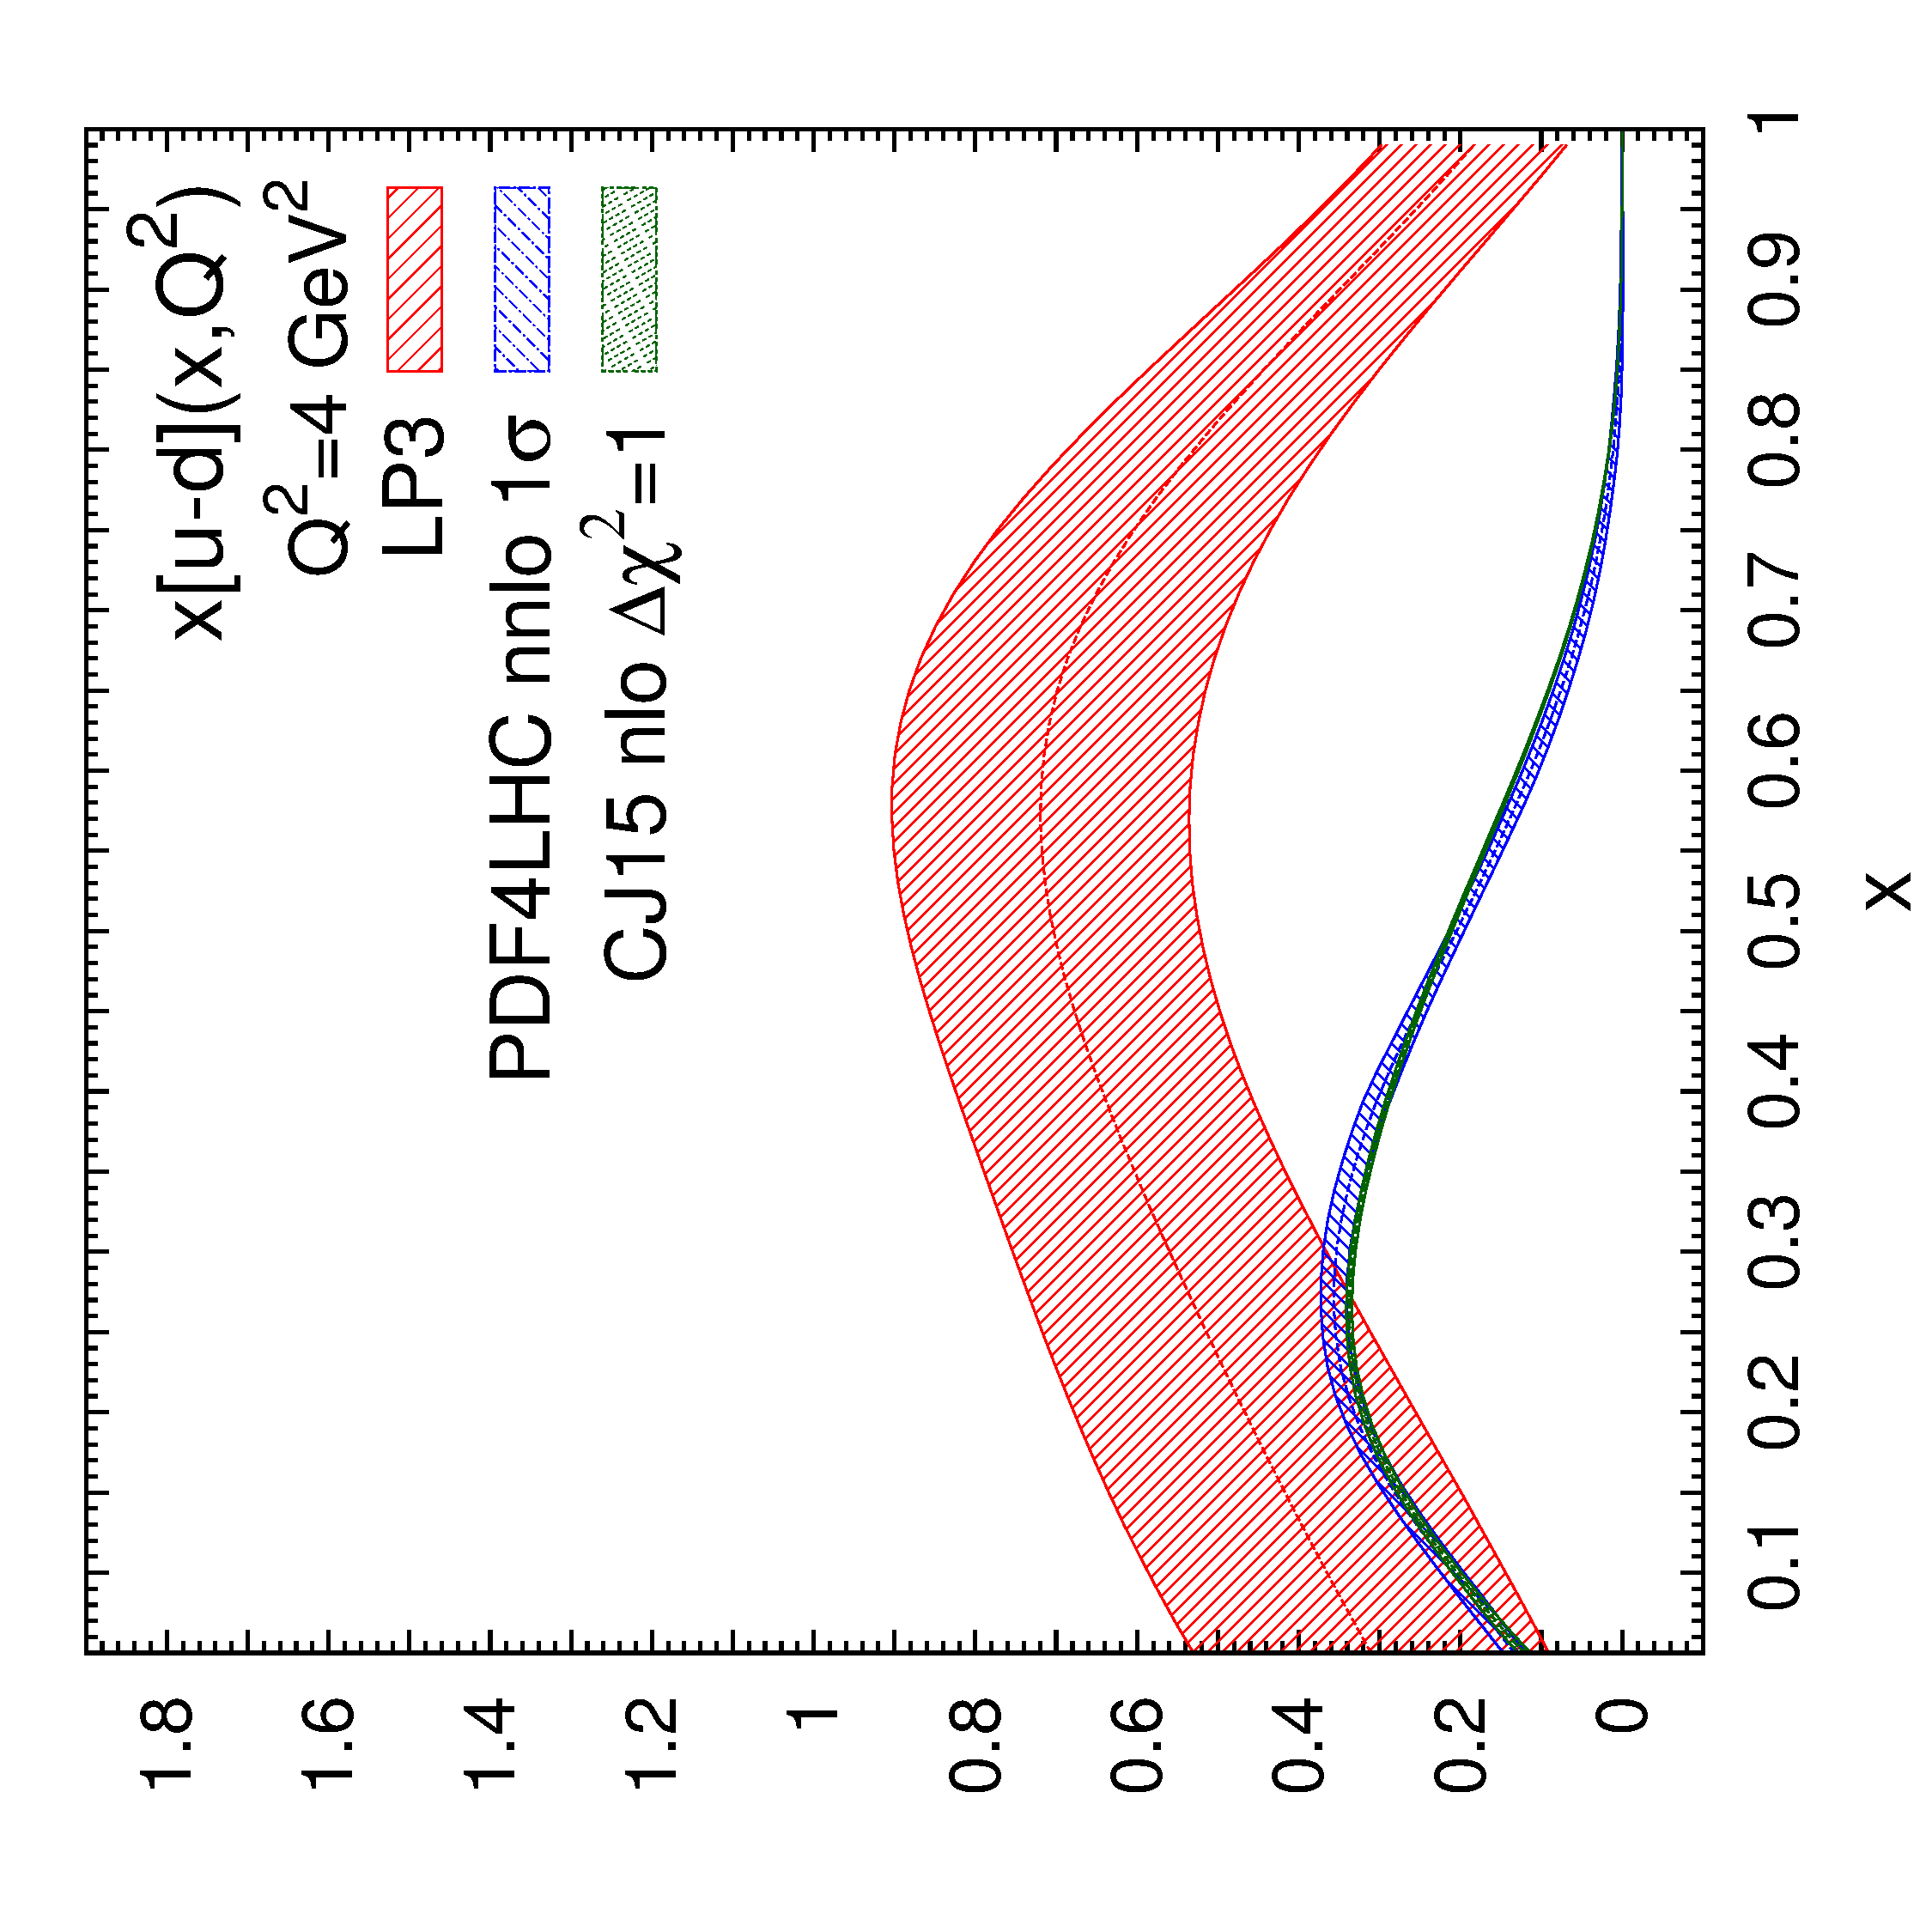
\includegraphics[scale=0.22,angle=270]{plots/unpxq}
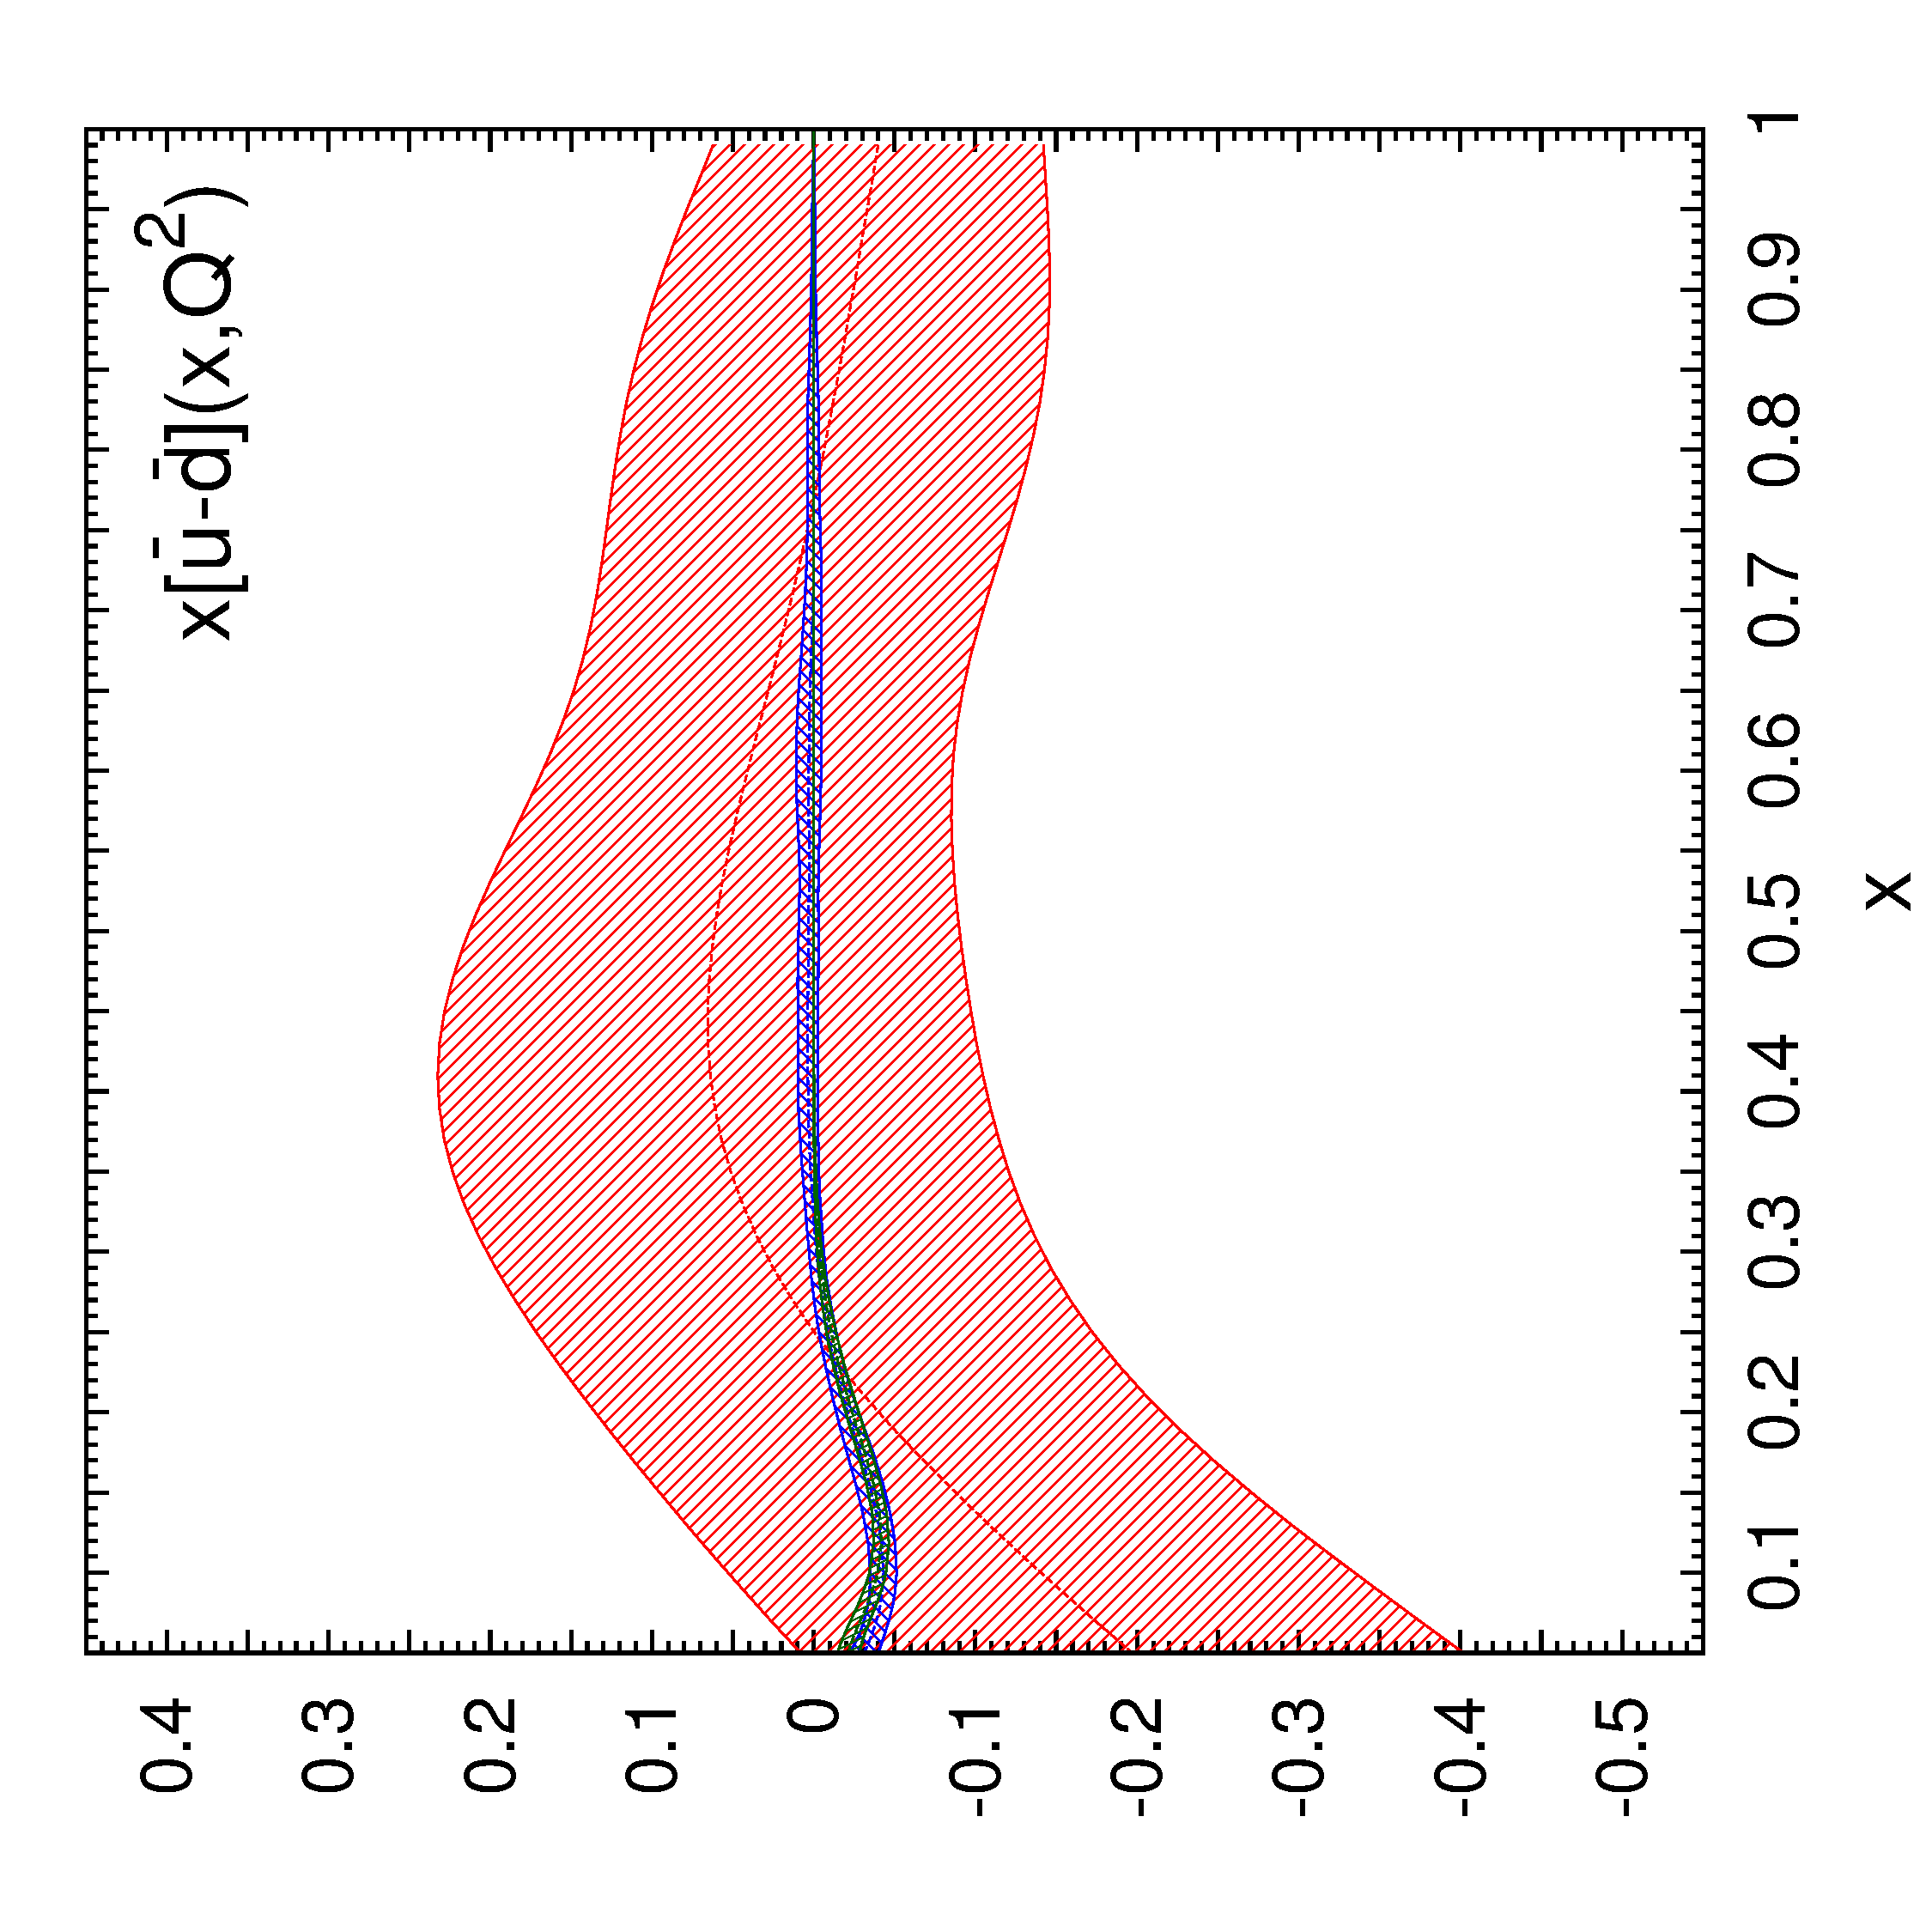
\includegraphics[scale=0.22,angle=270]{plots/unpxqbar}\\
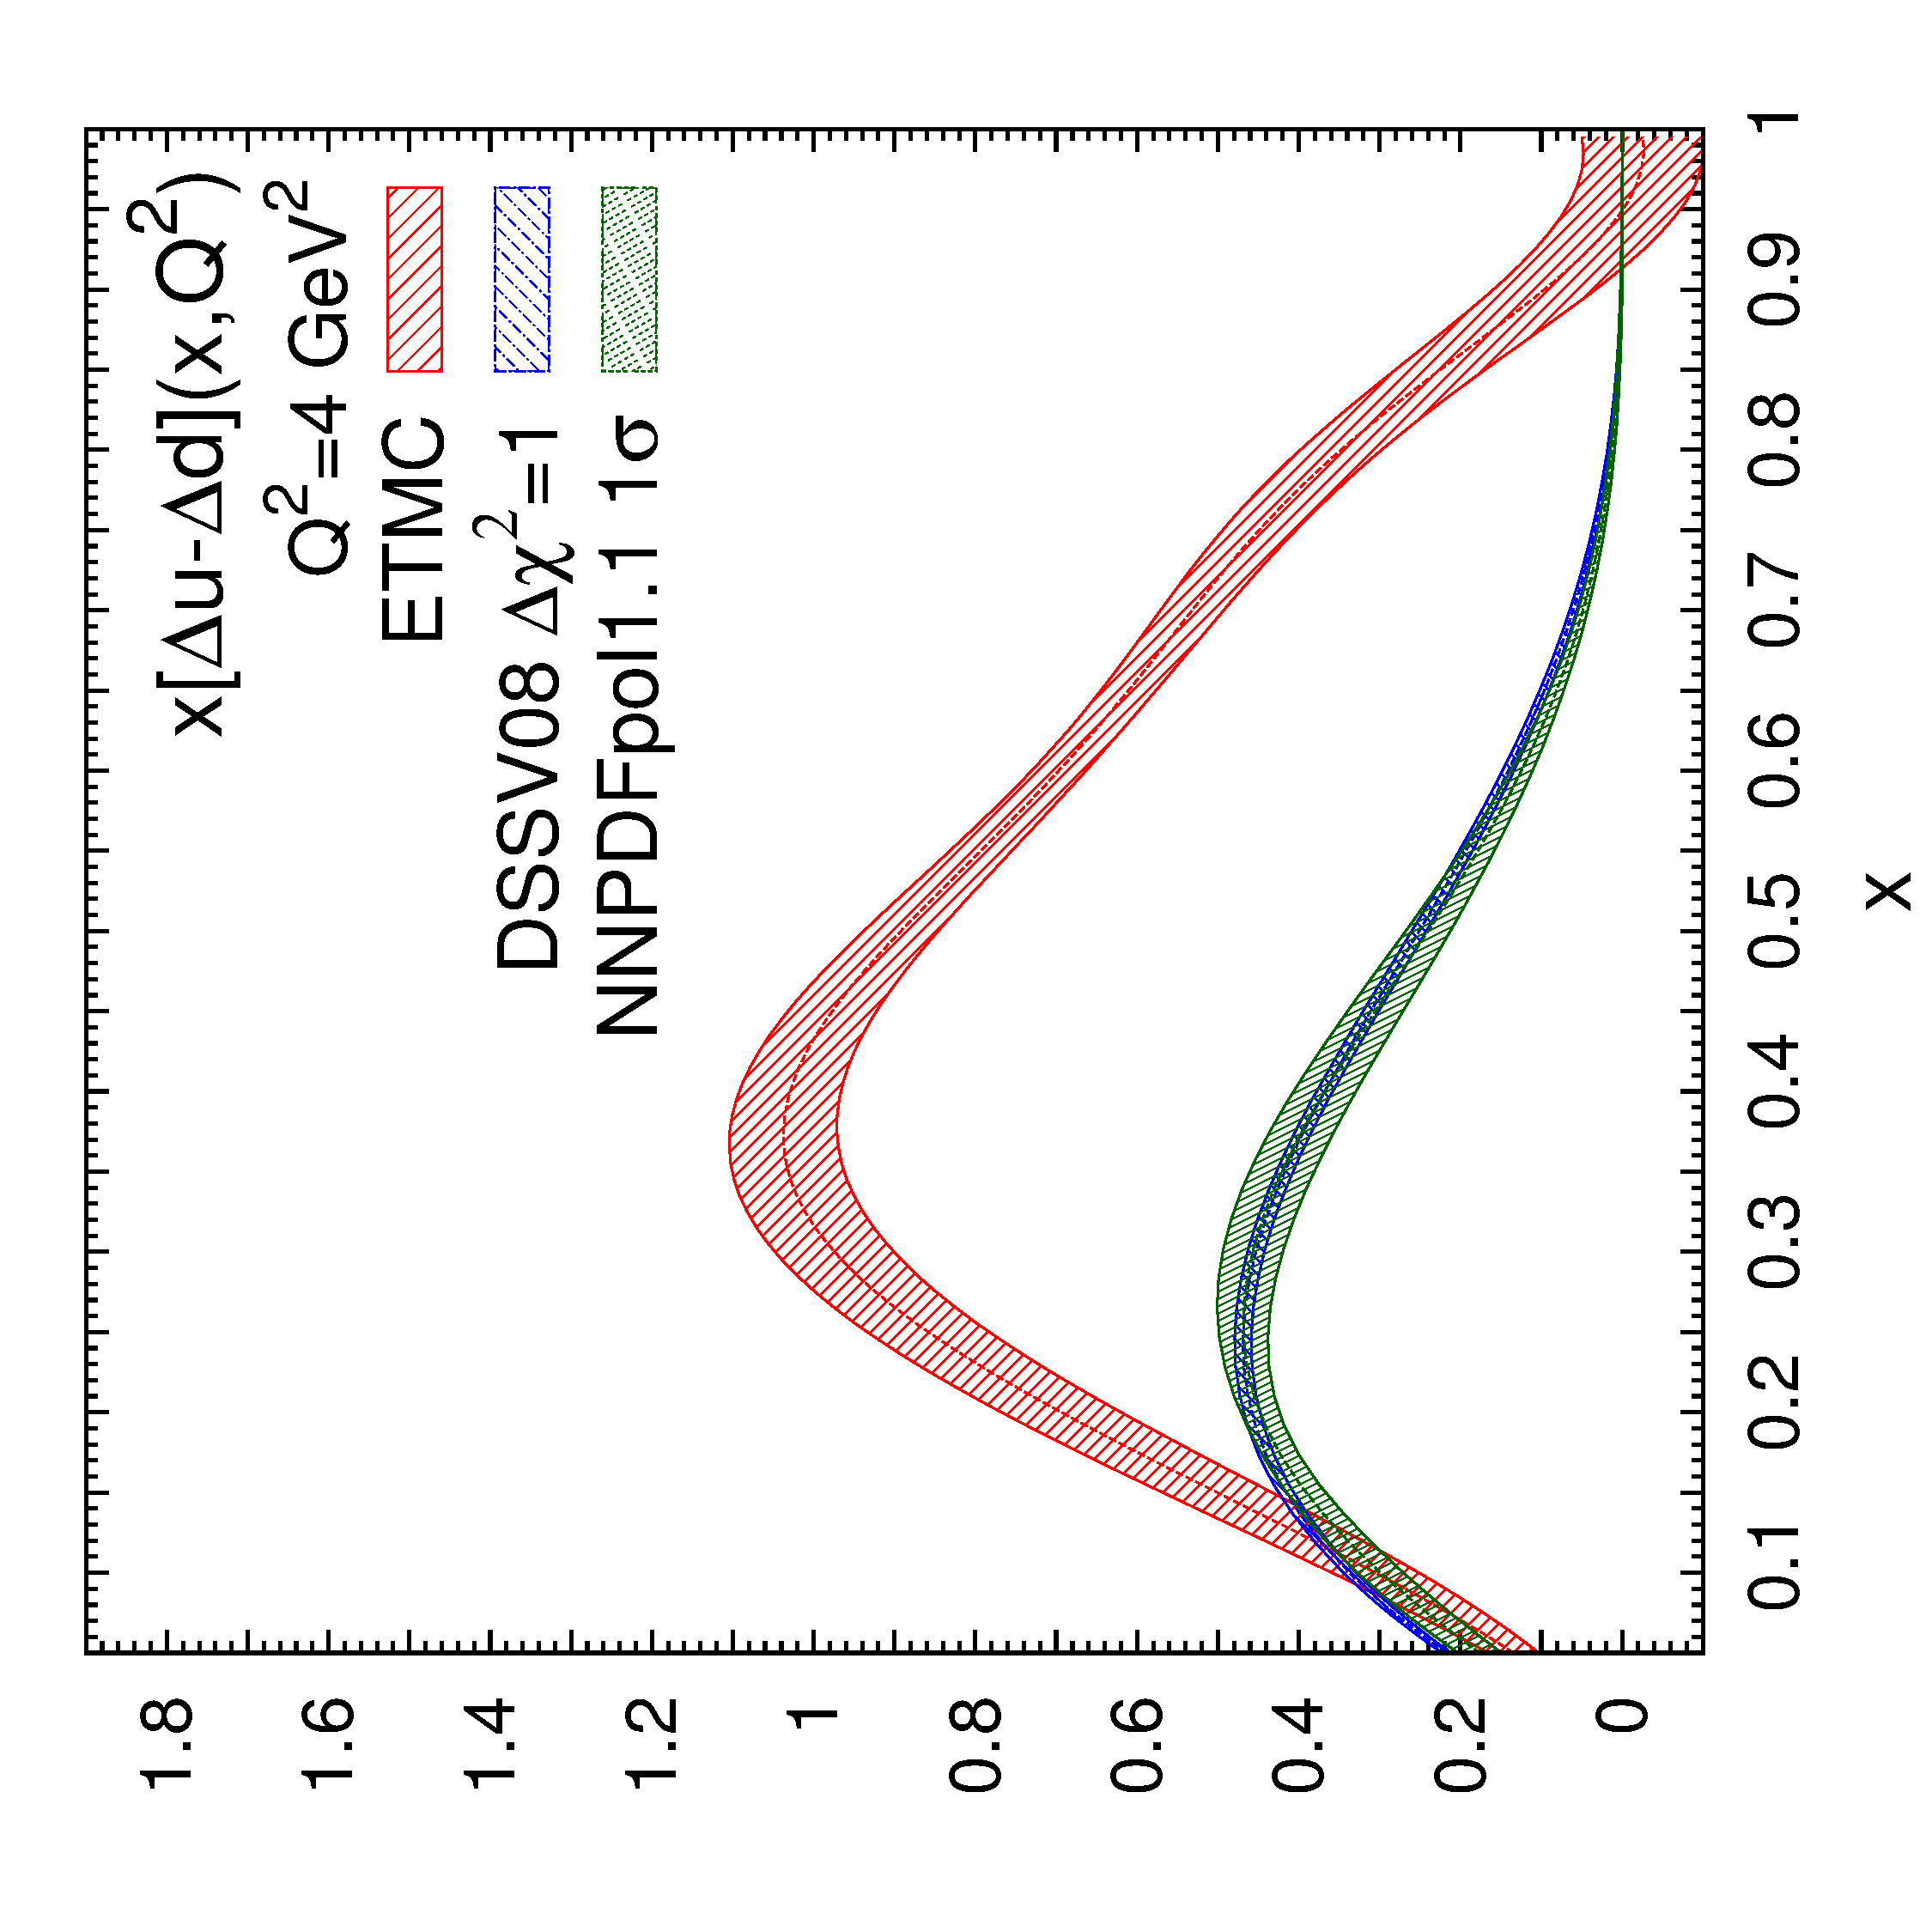
\includegraphics[scale=0.22,angle=270]{plots/polxq}
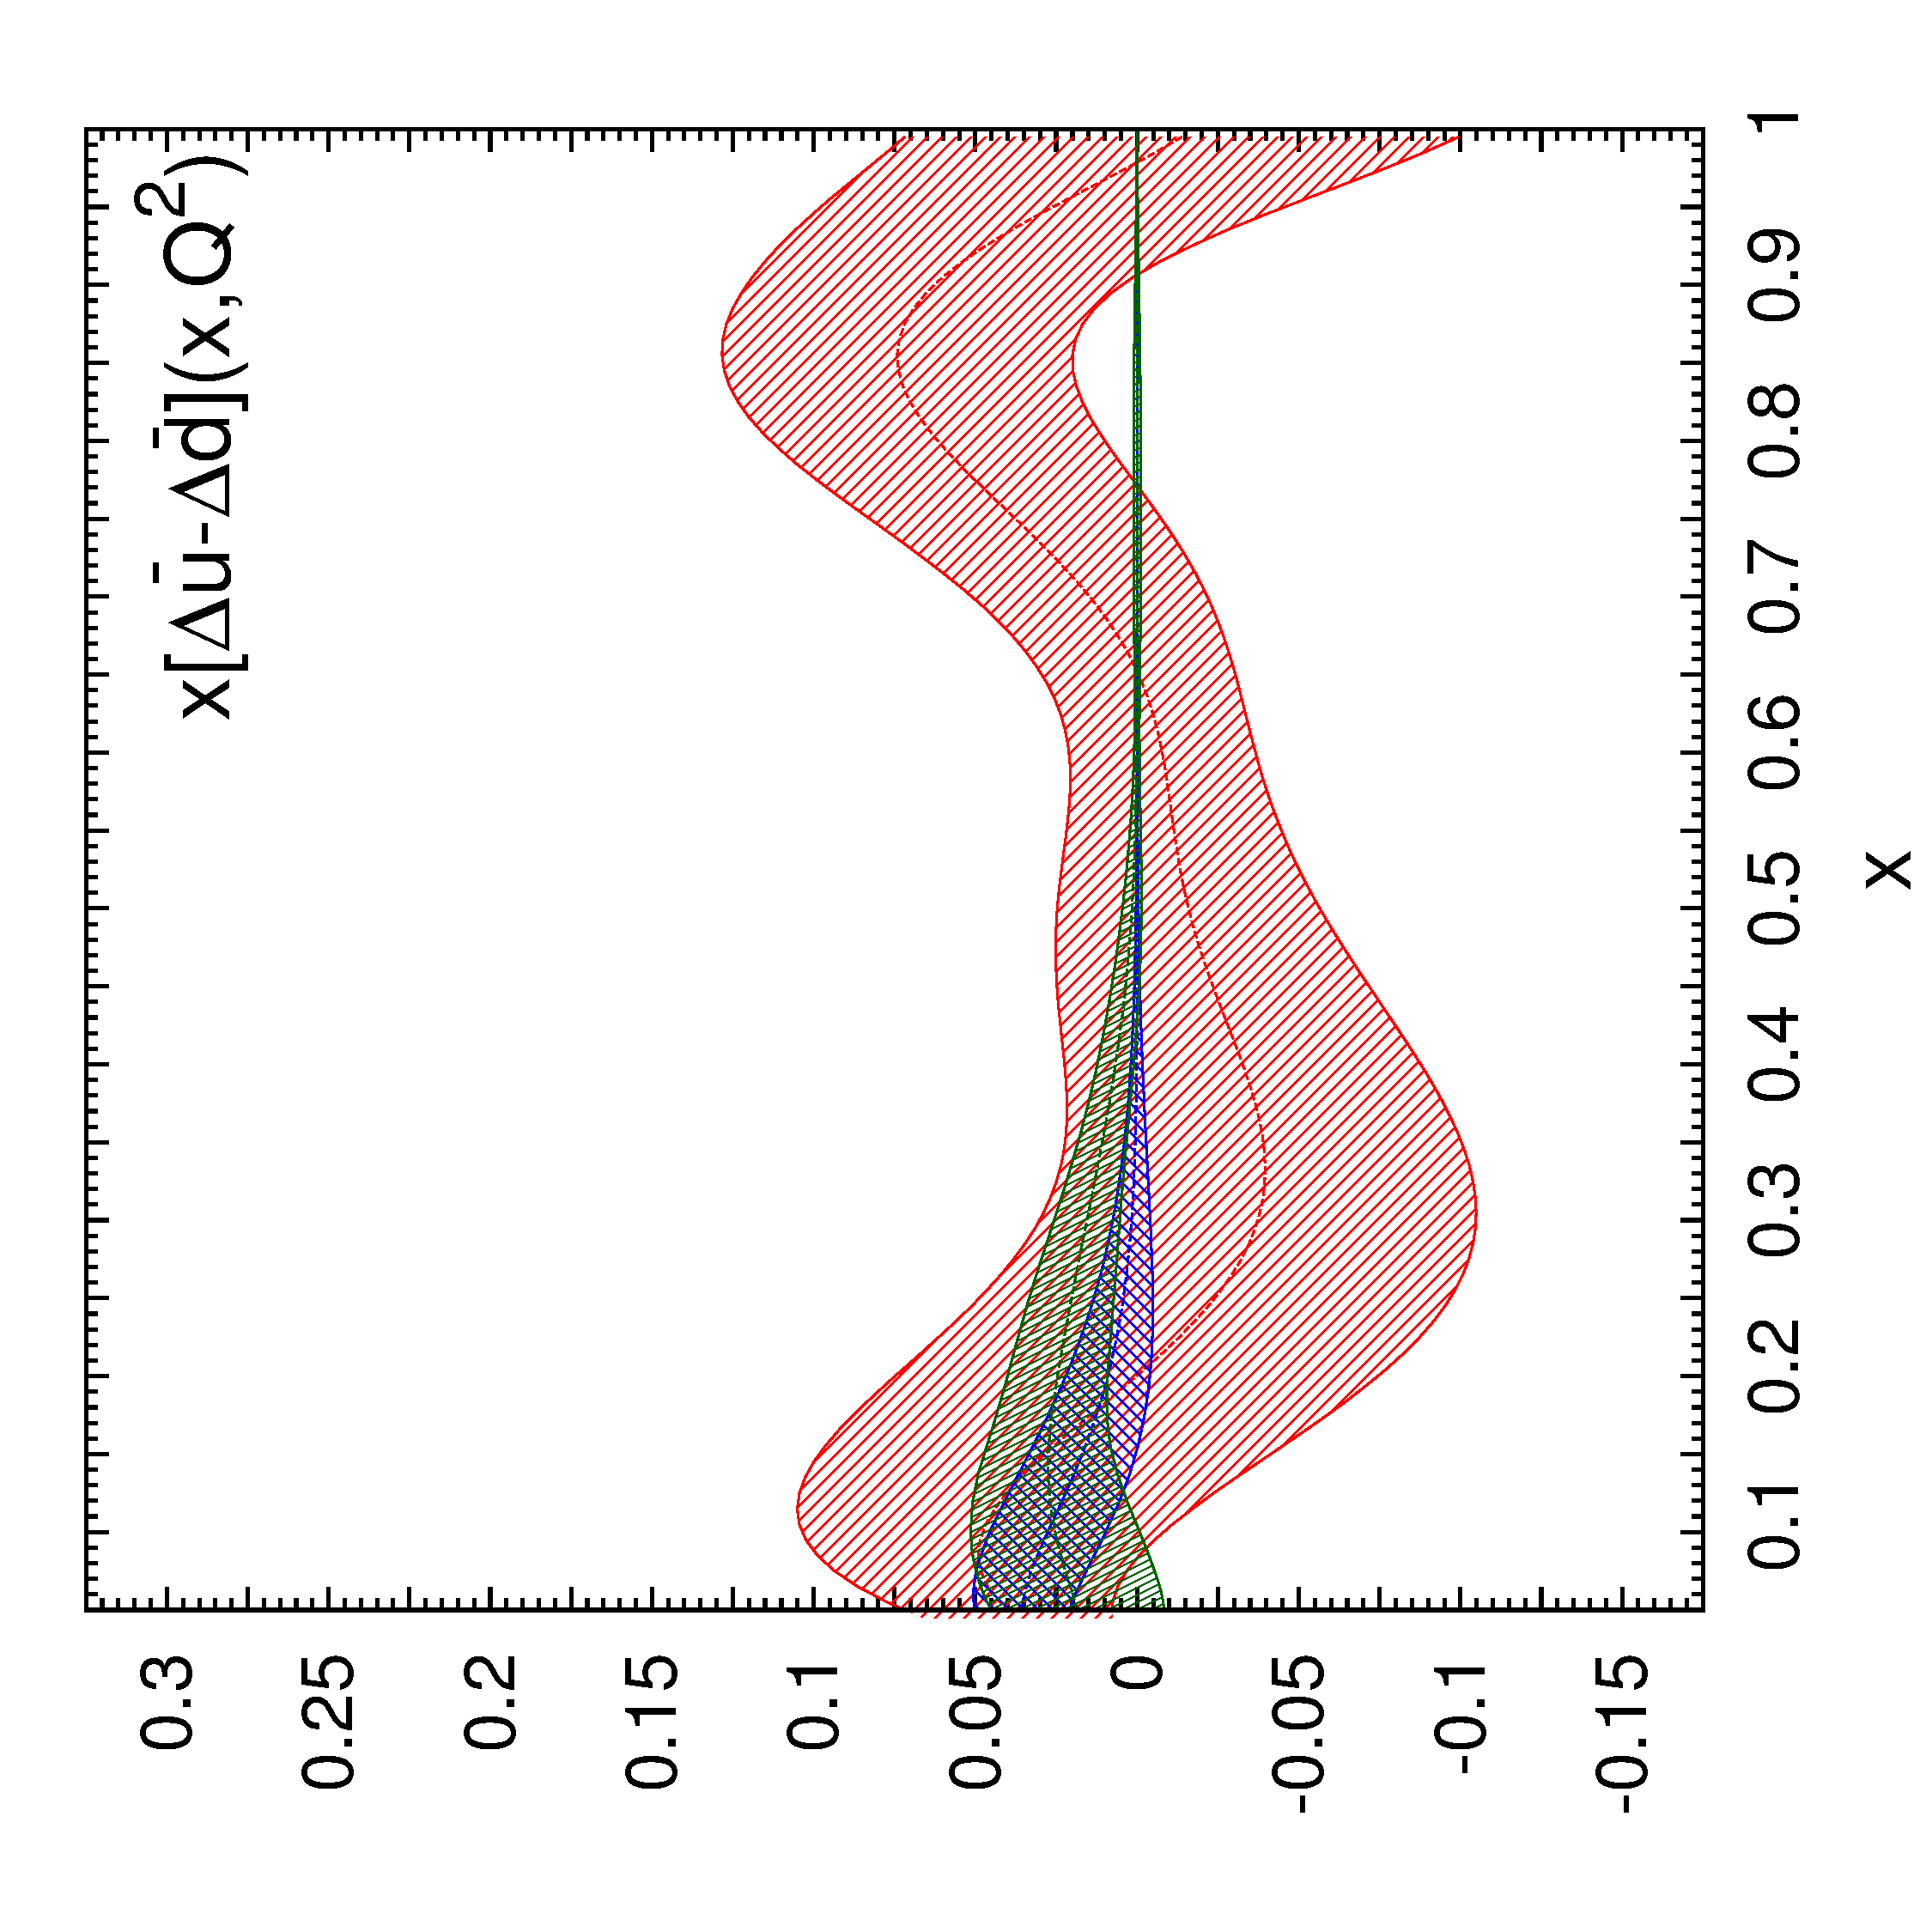
\includegraphics[scale=0.22,angle=270]{plots/polxqbar}\\
\caption{\small LP3's renormalised unpolarised isovector quark (top left) and 
  antiquark (top right) PDF combinations at pion mass of 310 MeV after 
  one-loop matching and mass correction at the renormalisation scale 
  $\mu=2$~GeV~\cite{Chen:2017mzz}. 
  %
  ETMC's renormalised polarised isovector quark (bottom left) and antiquark
  (bottom right) PDF combinations at pion mass of 
  375 MeV~\cite{Alexandrou:2017huk}.} 
\label{fig:qPDF-demo}
\end{figure}


\paragraph*{Pseudo-PDFs} 
The general dependence of the  matrix element $h(z,p_z)$ of Eq.~\eqref{eq:qPDF} 
on the hadron momentum $p$ and the displacement of the quark and anti-quark 
fields $z$ can be expressed as a function of the Lorentz invariants 
$\nu=z\cdot p$ (Ioffe time~\cite{Ioffe:1969kf,Braun:1994jq}) 
and $z^2$ where $z$  and $p$ is a general 4-vectors.  
%
We can thus introduce
\begin{equation}
\overline{h}(\nu,z^2) \equiv h(z,p_z)\,.
\end{equation}

The pseudo-PDF is then defined by the Fourier transform
%
\begin{equation}
{\mathcal P}(x,z^2)=\int \frac{d\nu}{2\pi} e^{-ix\nu} \overline{h}(\nu,z^2),
\end{equation}
which has support only in the physical range 
$x=[-1,1]$ \cite{Radyushkin:2016hsy,Radyushkin:2017cyf}. 
%
As discussed in~\cite{Radyushkin:2016hsy,Radyushkin:2017cyf}, the pseudo-PDF 
is directly related to both the PDFs as well as the primordial TMD that 
describes the transverse structure of the hadron.
%
In~\cite{Radyushkin:2017cyf}, using the temporal gamma matrix in the matrix 
element, a possible factorization of the TMD and PDF was conjectured which 
implies that the ratio
%
\begin{equation}
{\mathcal M}(\nu,z^2) =\frac{\overline h(\nu,z^2)}{\overline h(0,z^2)}
\label{eq:RatioPseudo}
\end{equation}
is directly related to PDFs as 
\begin{equation}
{\mathcal M}(\nu,z^2) =Q(\nu,z^2) + {\cal O}(z^2),
\label{eq:IoffePDF}
\end{equation}
with $Q(\nu,z^2)$ being the Ioffe time PDF~\cite{Ioffe:1969kf,Braun:1994jq} 
which is just the Fourier transform of the PDFs.
\begin{equation}
{q}(x,1/z^2)=\int \frac{d\nu}{2\pi} e^{-ix\nu} Q(\nu,z^2),
\end{equation}
Note, that the ratio in Eq.~\ref{eq:RatioPseudo} has a well defined continuum 
limit and requires no renormalization. 
%
The polynomial corrections in Eq.~\ref{eq:IoffePDF} are due to violations of 
the factorization conjecture, while the PDF ${q}(x,1/z^2)$ is the PDF in a 
particular scheme defined at scale $1/z^2$. Matching to $\overline{MS}$ 
can be performed in perturbation theory following standard methodology. 
%
One loop results are published in~\cite{Ji:2017rah}.
%
A preliminary study of this formalism was presented in~\cite{Orginos:2017kos}, 
where it was shown that indeed the conjectured factorization is observed and 
the residual corrections are small. Furthermore  evidence of the expected 
perturbative evolution of the Ioffe time PDFs was observed. 
%
More detailed studies of this methodology are required to achieve its full 
potential.  
